%%%%%%%%%%%%%%%%%%%%%%%%%%%%%%%%%%%%%%%%%%%%%%%%%%%%%%%
% A template for Wiley article submissions developed by 
% Overleaf for the Overleaf-Wiley pilot which ran 
% during 2017 and 2018.
% 
% This template is no longer supported, but is provided
% for historical reference. Last updated January 2019.
%
% Please note that whilst this template provides a 
% preview of the typeset manuscript for submission, it 
% will not necessarily be the final publication layout.
%
% Document class options:
% =======================
% blind: Anonymise all author, affiliation, correspondence
%        and funding information.
%
% lineno: Adds line numbers.
%
% serif: Sets the body font to be serif. 
%
% twocolumn: Sets the body text in two-column layout. 
% 
% num-refs: Uses numerical citation and references style 
%           (Vancouver-authoryear).
%
% alpha-refs: Uses author-year citation and references style
%             (rss).
%
% Using other bibliography styles:
% =======================
%
% To specify a different bibiography style
%
% 1) Do not use either num-refs or alpha-refs in documentclass.
% 2) Load natbib package with the options set as needed.
% 3) Use the \bibliographystyle command to specify the style
% 
% Included NJD styles are: 
%   WileyNJD-ACS
%   WileyNJD-AMA
%   WileyNJD-AMS
%   WileyNJD-APA
%   WileyNJD-Harvard
%   WileyNJD-VANCOUVER
%
% or you may upload an alternative .bst file 
% (if requested by the journal).
%
% Examples:
% =======================
%% Example: Using numerical, sort-by-authors citations.


\documentclass[num-refs]{wiley-article}
%% Example: Using author-year citations and anonymising submission
% \documentclass[blind,alpha-refs]{wiley-article}

%% Example: Using unsrtnat for numerical, in-sequence citations
%\documentclass{wiley-article}
%\usepackage[numbers]{natbib}
%\bibliographystyle{unsrtnat}

%Citation style from another project
%\usepackage[citestyle=numeric,style=numeric,backend=biber]{biblatex}
%% Example: Using WileyNJD-AMA reference style and superscript
%%          citations, two-column and serif fonts for AIChE
%\documentclass[serif,twocolumn,lineno]{wiley-article}
%\bibliographystyle{WileyNJD-AMA}
% \makeatletter
% \renewcommand{\@biblabel}[1]{#1.}
% \makeatother

% Add additional packages here if required
\usepackage{natbib}
\usepackage{siunitx}
\graphicspath{{./images/}}
\usepackage{wrapfig}
% Update article type if known
\papertype{Original Article}
% Include section in journal if known, otherwise delete
\paperfield{Organic chemistry synthesis}

\title{Synthesis of \texorpdfstring{H\textsubscript{2}}-TPP and its metallation to Zn-TPP}

% List abbreviations here, if any. Please note that it is preferred that abbreviations be defined at the first instance they appear in the text, rather than creating an abbreviations list.
\abbrevs{\texorpdfstring{H\textsubscript{2}}-TPP, 5,10,15,20-meso-tetraphenylporhyrin.}

% Include full author names and degrees, when required by the journal.
% Use the \authfn to add symbols for additional footnotes and present addresses, if any. Usually start with 1 for notes about author contributions; then continuing with 2 etc if any author has a different present address.
\author[1\authfn{1}]{Matteo Finco*, Nicola Milani}


% Include full affiliation details for all authors
\affil[1]{DiSC, Università degli Studi di Padova, Padova, Italy, 35131, Italy}

\corremail{matteo.finco.3@studenti.unipd.it}
% Include the name of the author that should appear in the running header
\runningauthor{Matteo Finco}

\begin{document}

\begin{frontmatter}
\maketitle

\begin{abstract}
    Tetraphenylporhyrin and Zn-TPP are characterized by a robust aromatic structure, interesting optical properties but their synthesis require time and extensive use of solvents while leading to moderate yields.
    A Rothemund synthesis was adopted and the monitoring through TLC of the reaction state allowed to recognize that the reaction is actually happening in a much shorter time than expected.
    Product characterizations through $^{1}$H NMR and ESI-MS are discussed as well as the application of Zn-TPP as photosensitizer in resins for 3D printing.

% Please include a maximum of seven keywords
\keywords{tetraphenylporphyrin,H$_{2}$-TPP, Zn-TPP,$^{1}$H NMR, ESI-MS, LED projector 3D printing}
\end{abstract}

\end{frontmatter}

\section{Introduction}
\begin{wrapfigure}{L}{0.35\textwidth}
    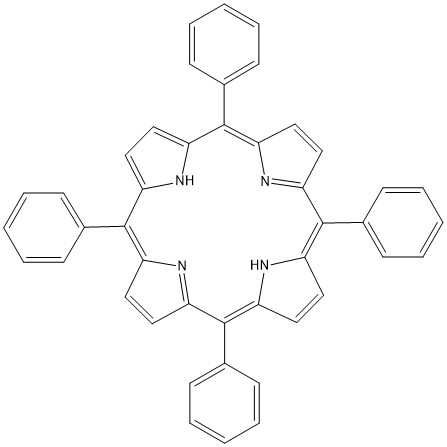
\includegraphics[width=0.3\textwidth]{TPP}
    \caption{TPP structure}
    \label{TPP-structure}
\end{wrapfigure}
Porhyrins represent an obiquitous class of molecules that plays a crucial role biochemistry for oxygen transport\citep{hardison_evolution_2012}, storage\citep{kendrew_three-dimensional_1958} and catalysis as well as electron transfer\citep{keilin_cytochrome_1925}.\\
Therefore, extensive efforts have been put into the exploration of the functionalities obtainable by artificially synthesized porphyrins.\\
The biomimetic electrocatalysis\cite{facchin_oxygen_2021,liang_porphyrin-based_2021} and cancer treatment and diagnosis\cite{wang_recent_2021} represent two outstanding examples among all the use cases in which porphyrins have been successfully deployed.
Numerous works elaborate the further functionalization of \textit{meso}-tetraphenylporphyrin\cite{silva_porphyrins_2006} in order to realize functional materials. \\
However, to date the scale up in complex porphyrins production and broad commercial application is prevented by the production costs which are primarily led up by the expensiveness of reactants, inefficient and unreliable synthesis.
In the following work, a simple synthesis route for 5,10,15,20-mesotetraphenylporhyrin is detailed and its products are critically discussed either for the \texorpdfstring{H\textsubscript{2}}-TPP and the metallated Zn-TPP.

\newpage

\twocolumn
\section{Methods}
\begin{figure*}[t!]
        \centering
        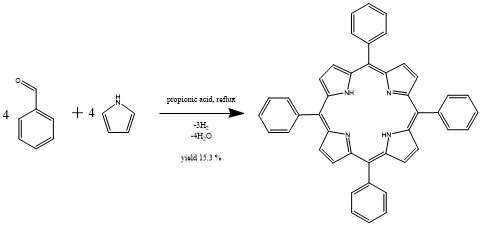
\includegraphics[width=0.6\textwidth]{reaction}
        \caption{Reaction scheme for \textit{meso}-TPP synthesis through condensation in acidic medium.}
        \label{reaction}
\end{figure*}
The synthesis proposed for \textit{meso}-tetraphenylporphyrin is a multistep electrophilic aromatic substitution between the electrophilic carboxilic group of protonated benzaldehyde on the aromatic ring of pyrrole which is summarized in Fig.\ref{reaction}.
The protonation of benzaldehyde implies that the reaction is performed in acidic environment, and its protonated form is stabilized by the resonance forms reported in Fig.\ref{res-benz}.\\
\begin{figure*}[b!]
    \centering
    \begin{subfigure}
        \centering
        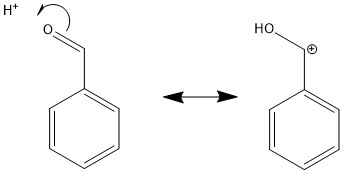
\includegraphics[width=0.3\textwidth]{resonance-benzaldehyde}
        \caption{Resonance forms of benzaldehyde in acidic environment.}
        \label{res-benz}
    \end{subfigure}
    \begin{subfigure}
        \centering
        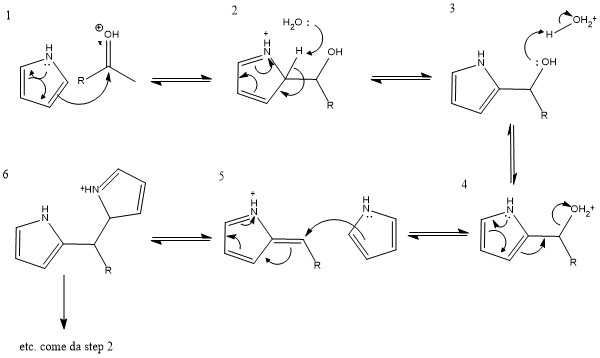
\includegraphics[width=0.5\textwidth]{mechanism}
        \caption{Reaction mechanism for electrophilic substitution on the pyrrolic ring by aldehyde groups.}
        \label{mechanism}
    \end{subfigure}
\end{figure*}
This route is called Rothemund synthesis and proceeds through the repetition of the six steps in Fig.\ref{mechanism} thanks to the driving force provided by the stability of the wide aromatic system.
The reaction consists in multiple condensations occurring at the addition of each unit to the porhyrinic ring.
The first step consist in the electrophylic attack of the protonated aldehyde to the pyrrolic ring.
Then, the pyrrolic ring extracts the positive charge and gets deprotonated in the second step.
The re-protonation of the carbonilic group by the acidic environment forms the leaving group -OH$_{2}$$^{+}$ which causes the condensation of the reagents and the relocaliization of the positive charge on the nitrogen atom by the misplacing of its lone pair into the pyrrolic ring.
The methynic bridge is instaurated by the electrophyle attack of the insaturated bond and the concerted relocation of the positive charge into the newly added pyrrolic ring.
\break
The metallation of the free base porhyrin is operated by the reaction in reflux conditions with zinc acetate as reported in Fig. \ref{metalation}.
\begin{figure*}
    \centering
    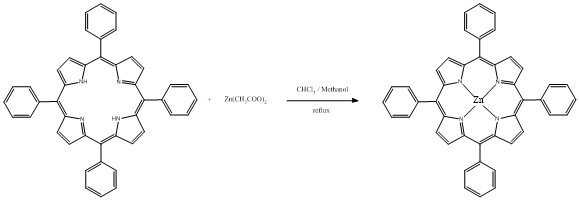
\includegraphics[width=0.8\textwidth]{Zn-TPP reaction}
    \caption{Reaction scheme for the metallation of the free base porphyrin.}
    \label{metalation}
\end{figure*}
The use of chloroform is necessary for the solvation of the freebase porphyrin, while methanol solvates the zinc acetate.
The metallation of the free base porphyrin is allowed by its deprotonation which is promoted by the basic behaviour of the acetate anion.
Then, the Zn(II) cation is coordinated by the four nitrogen atoms.
It is important to perform the metallation with an excess of zinc acetate in order to promote the consumption of the limiting reagent, which should be the free base TPP.\\

%%%%%%%%%%%%%%%%RESULTS AND DISCUSSION%%%%%%%%%%%%%%%

\section{Results and Discussions}
In the following section, the characterization results are presented and discussed for both, the free base and the metallated porphyrin.
\subsection{\textit{In operando} characterizations}
The reactions were monitored using Thin Layer Chromatography.
In Fig. \ref{tlc-h2tpp} it is possible to see that the reaction already had occurred by the time of the first control, which corresponds to around 5 minutes of reaction time.
This can be affirmed since the control TLC performed after 30 minutes of reaction time also against a commercial standard, exhibited the same features.
It must be noted that the R$_{f}$ of the tested samples appear to shift to higher values.
The reason of which might be found in two possible phenomena, namely the change in eluent composition due to higher vapor pressure of petroleum ether compared to methanol and the excessive eluent run that was performed on the second plate.
Indeed, the fact that the second plate had the eluent almost to its edge might have caused a distortion of the R$_{f}$ in excess.
In the meanwhile, the instability in composition of the eluent might explain the shift in relative differences of the R$_{f}$ coefficients between benzaldehyde and pyrrole, since their difference in R$_{f}$ changes from 14\% to 9\%.

At the end of the synthesis, the yield was estimated to be 15.3\%, which amounted to the synthesis of 0.339 g of product against the 2.21 g expected if the reaction had been quantitative and limited by pyrrole, the limiting reactant.
The metallation of the free base porphyrin was monitored once again by the use of TLC plates 2, 5 and 25 minutes since the beginning of the reaction.
The results of which can be observed in the Fig.\ref{TLC-Zn-TPP}.\\
Also in this case the yield has been quantified by weighting on a digital scale a vial before and after the addition of the last product.
Nevertheless, the result is meaningless since the theoretical yield was 208 mg and the weighted substance exhibited a mass of 434 mg.
The reason for this inconvenience might consist on permaining unreacted products, impurities or water.
\begin{figure*}[t!]
    \centering
    \begin{subfigure}
        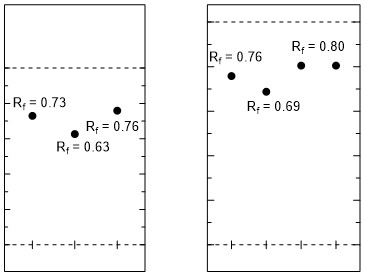
\includegraphics[width=0.3\textwidth]{TLC-h2-TPP}
        \caption{On the left, the TLC run performed 5 minutes after the addition of the reagents to the flask.
        The spots from left to right are corresponding to benzaldehyde, pyrrole and the reaction solution.
        On the right, the TLC run performed 30 minutes after the addition of the reagents to the flask.
        The spots from left to right are corresponding to benzaldehyde, pyrrole, commercial H$_{2}$-TPP and the reaction solution.}
        \label{tlc-h2tpp}
    \end{subfigure}
    \begin{subfigure}
        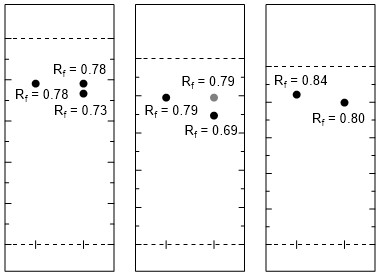
\includegraphics[width=0.3\textwidth]{TLC-Zn-TPP}
        \caption{The spots are corresponding to the prepared H$_{2}$-TPP on the left and the reaction solution on the right, respectively sampled 2, 5 and 25 minutes after the beginning of the reaction.}
        \label{TLC-Zn-TPP}
    \end{subfigure}
\end{figure*}
Nevertheless, it is possible to conclude from the TLC plates that both the reactions followed a rather rapid course.
Considering that the yield obtained from the first reaction is well within the expected one for the Rothemund reaction (10 \% to 20 \%), we can state that the overall synthesis could potentially be performed in a much quicker manner.
This conclusion, opens up prospectives for further study.
Ideally, these study should also concentrate on the reduction of solvents employed in order to widen the application landscape of porphyrins.

%%%%%%%%%% Presentation of results obtained by other studies
\subsection{\textit{$^{1}$H NMR} characterization}
%Discussing the results of NMR --- Spectra and motivations
For this analysis, the spectra found in the work of \citet{anjali_zinc-tetraphenylporphyrin_2020} has been used as a literature source for displaying the interpretation of NMR spectra.
It must be pointed out that they incorrectly assign the \textbf{b} and \textbf{d} positions, therefore the presented spectra have been amended.
The execution of $^{1}$H NMR on the expected free base TPP returned five main signals (see Fig.\ref{NMR}), which are attributed as follows.
The most shielded at -2.713 ppm is attributed to NH protons, due to the electronrich character of the pyrrolic ring. 
In addition, its absence of multiplicity suggests the absence of hydrogen atoms in neighbouring positions, a condition that is only verified by NH protons in the structure of the target TPP.
The remaining peaks are all placed in the aromatic region.
The attributions indicated are based on the idea that the proximity to the porphyrin ring removes shielding, in order to distinguish b and c positions, and that pyrrolic protons have a higher shift than the phenyl ones, allowing the attribution of the d proton signal.
The integrated signals confirm once more the attribution of signals, since the \textbf{b} positions are in 3/2 with the ones in \textbf{c} and \textbf{d} positions.
It is noticeable that the slight shift difference expected between protons placed in the phenyl ring in \textit{meta} and \textit{para} positions, doesn't allow an effective discrimination of the two contributions.
Finally, it is noted that TMS is found in very close proximity to its expected shift of 0.
The fact that the features found can all be interpreted by the expected signals, suggest a good degree of purity of the synthesized compound and that the target synthesis was performed successfully.\\
Similarly, the spectrum of the product of metallation has been studied by $^{1}$H NMR, see Fig.\ref{NMR}.
In this case, the very same peaks are observed, besides the ones corresponding to the NH protons.
This allows to verify that protons have been removed completely from that position, but doesn't allow to verify the presence of Zn atoms coordinated by the porphyrinic system.
\begin{figure}
    \centering
    \begin{subfigure}
        \centering
        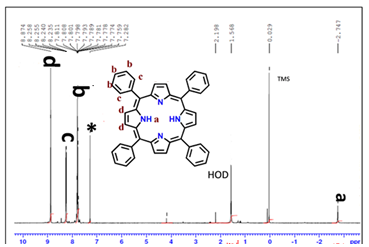
\includegraphics[width=0.45\textwidth]{1H-NMR-H2-TPP}
    \end{subfigure}
    \begin{subfigure}
        \centering
        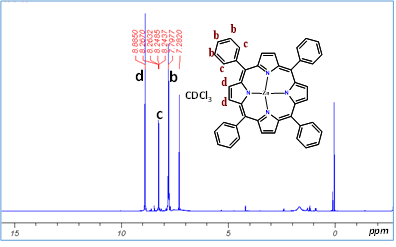
\includegraphics[width=0.5\textwidth]{1H-NMR-Zn-TPP}
    \end{subfigure}
    \caption{(\textit{above})$^{1}$H-NMR of H$_{2}$-TPP in TMS and (\textit{below}) Zn-TPP in chloroform.}
    \label{NMR}
\end{figure}
%%%%%%%%%%%%%%%%%%%%%%%%%%%%%%%%%%%%%%%%%%%%%%%%%%%%%%%%%%%%%%%%%%%%%%%%%%%%%%%%%%%%%%%%%%%%%%%%%%
\subsection{\textit{ESI-MS} characterization}
%Discussing the results of MS --- Spectra and motivations
For this section, the data collected and elaborated by previous students have been discussed.
Electrospray Ionization Mass Spectrometry (ESI-MS) was used to verify the presence of the target molecules in the product.
The observed peaks around the fundamental mass of each target molecule are studied to recognize the isotopic pattern of the atomic species.
Firstly, the spectra from the free base porphyrin has been superimposed to a simulated spectra as reported in Fig.\ref{ESI-MS-H2-TPP}.
It is observed that the position and relative intensity of the first three peaks is well reconstructed by the simulation.
However, the last peaks observed experimentally is heavily suppressed in the simulation.
This might suggest the presence in solution of a protonated TPP, H$_{3}$-TPP$^{+}$, which doesn't get ionized in the mass spectrometer.
The proposed scenario is the most likely to be true since protonated porphyrins are stable in presence of stronger acids.
Additionally, further protonations would lead to observe a \textit{m/z} half of the molecular mass of the TPP ring.
Conclusively, the FWHM of the experimental spectra well represent the widening effect due to the non-idealities introduced by the instrumental setup.\\

Secondly, the spectra elaborated from the data referring to Zn-TPP was plotted in Fig. \ref{ESI-MS-Zn-TPP}.
In this case, the isotopic pattern linked to the presence of Zn, is representative of the observed experimental features.\\
Therefore, these two investigations lead to successfully identify the presence of the targert molecules, validating the findings of the \textit{$^{1}$H NMR} characterization.
\textit{Please, mind that these characterizations are referring to different samples. None of which being the one realized by the students writing this report.
The last sentence is aimed to explicitate how different characterization techniques return information that can cooperatively ensure the correctness of data interpretation.}
\begin{figure}
    \centering
    \begin{subfigure}
        \centering
        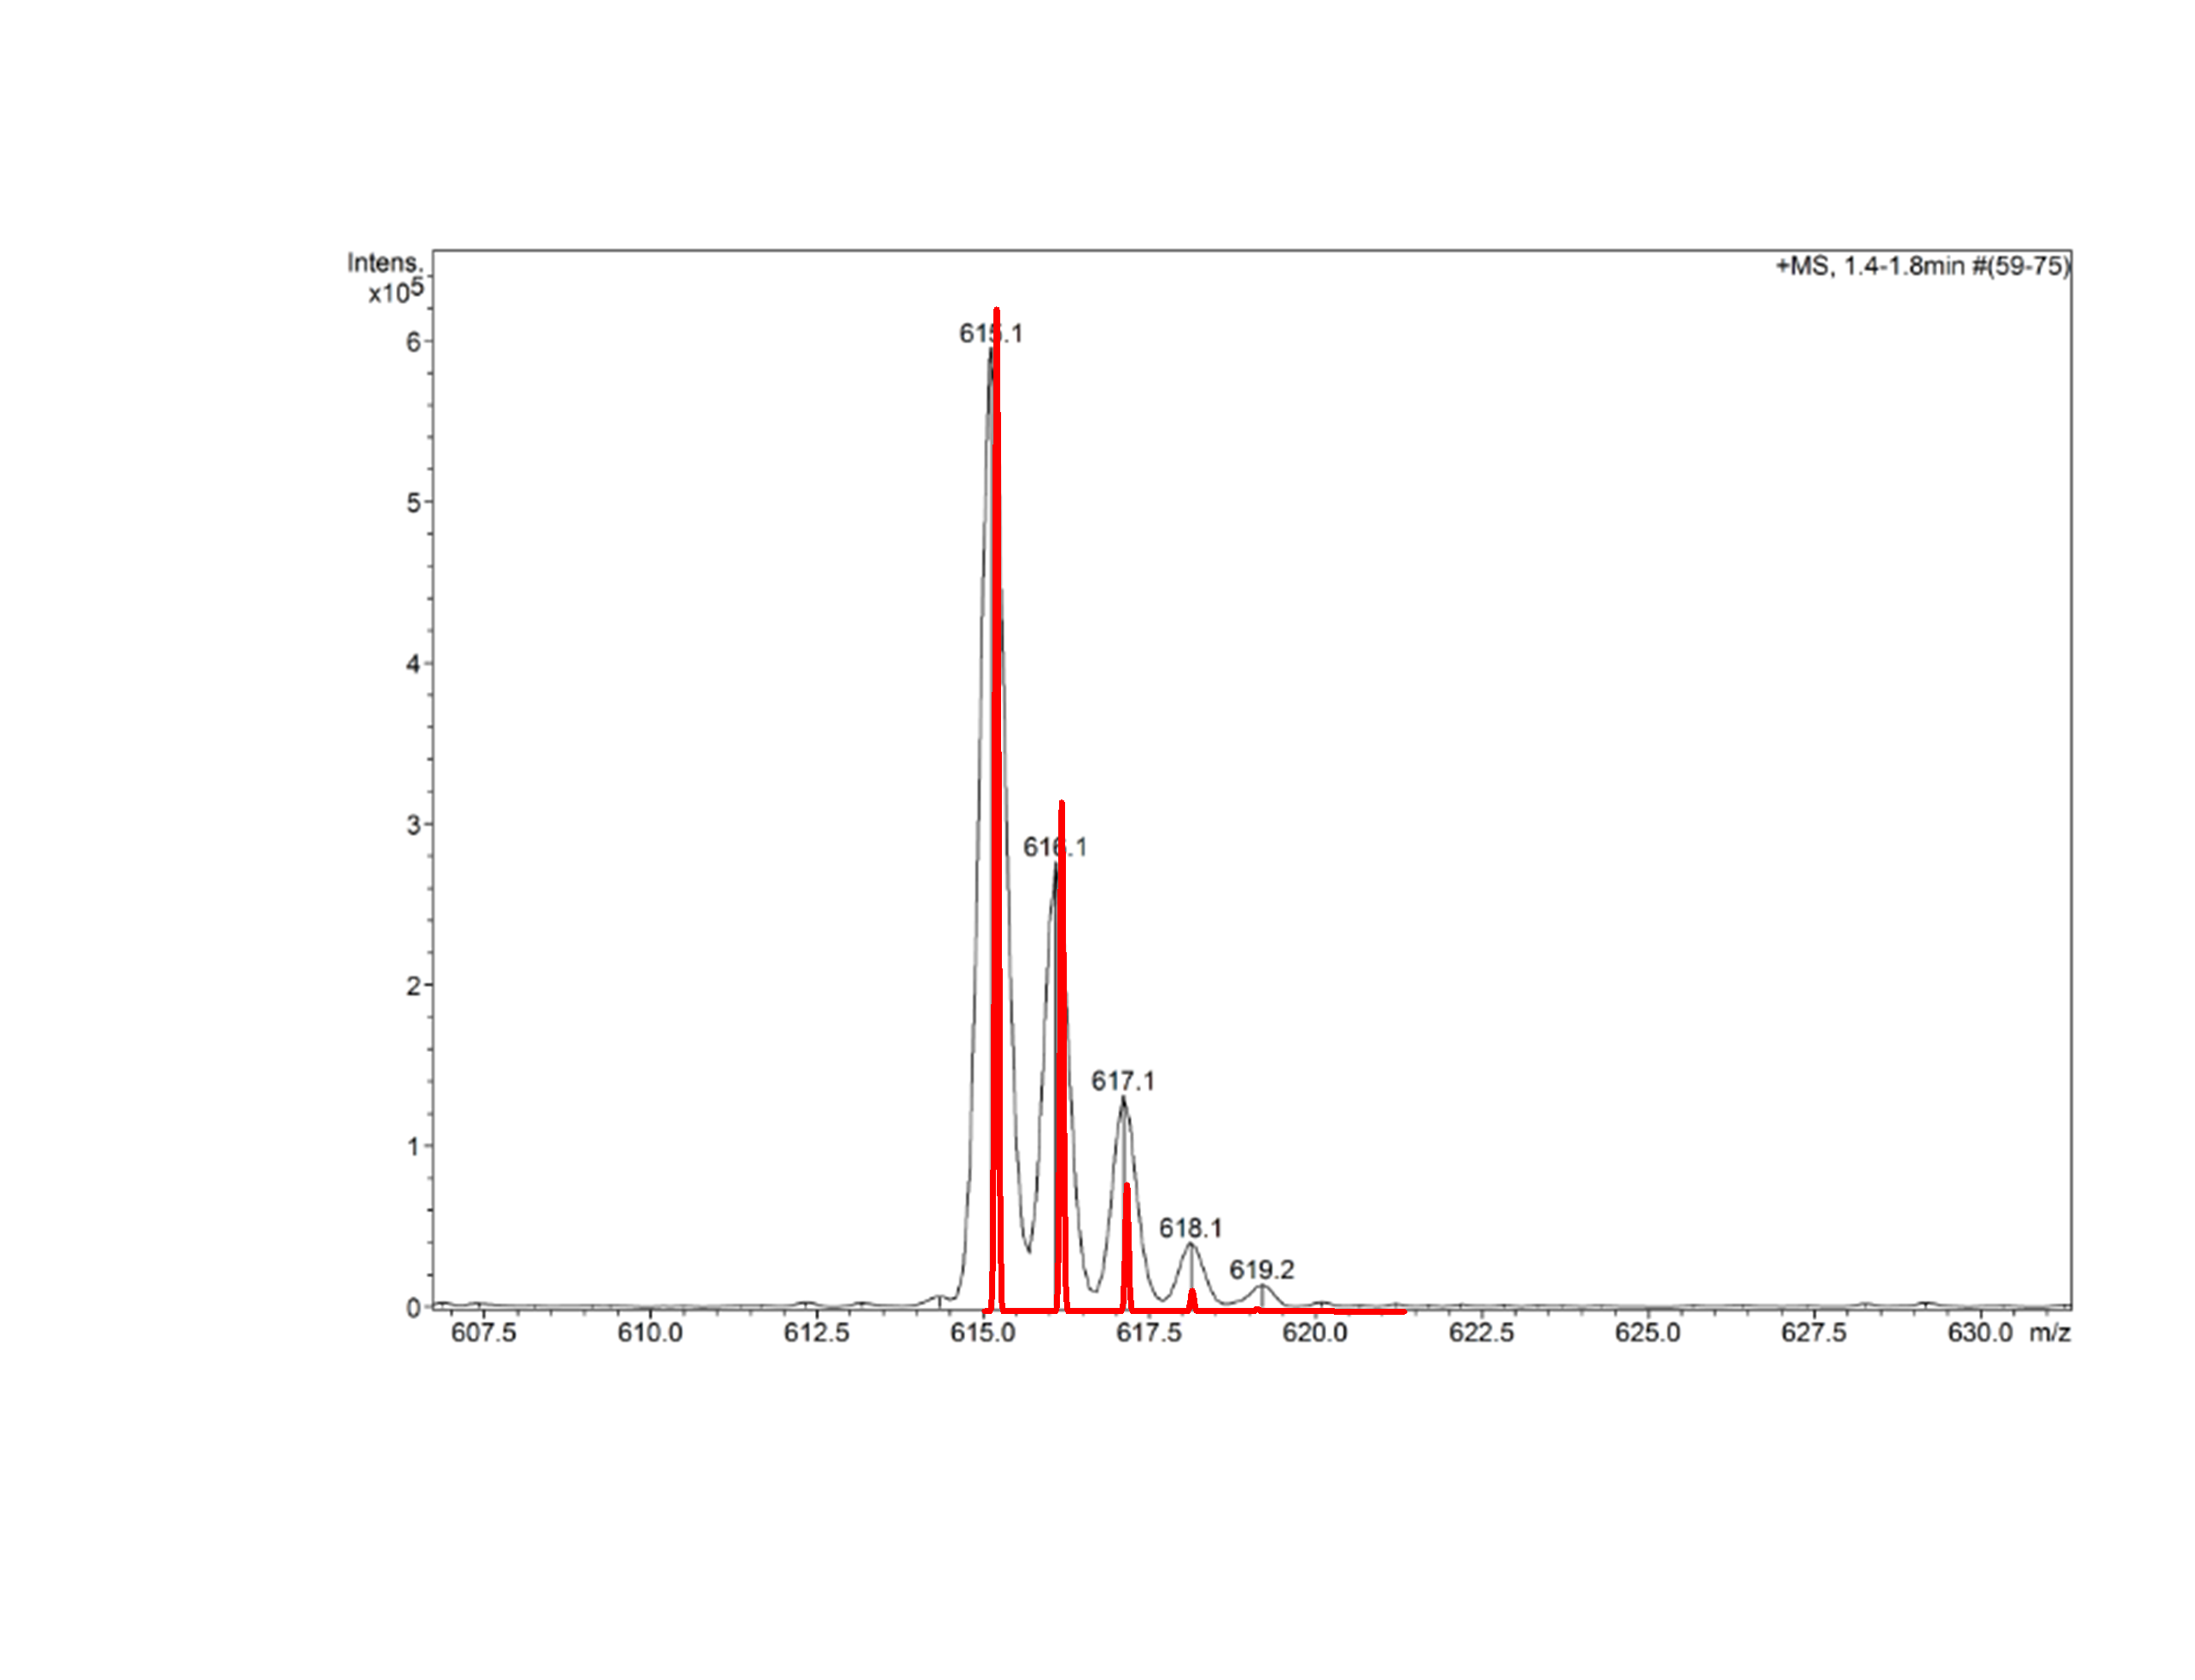
\includegraphics[width=0.45\textwidth]{ESI-MS-H2-TPP}
        \caption{ESI-MS of H$_{2}$-TPP around the main peak corresponding to the unfragmented molecular mass. The predicted spectra is reported as a red line.}
        \label{ESI-MS-H2-TPP}
    \end{subfigure}
    \begin{subfigure}
        \centering
        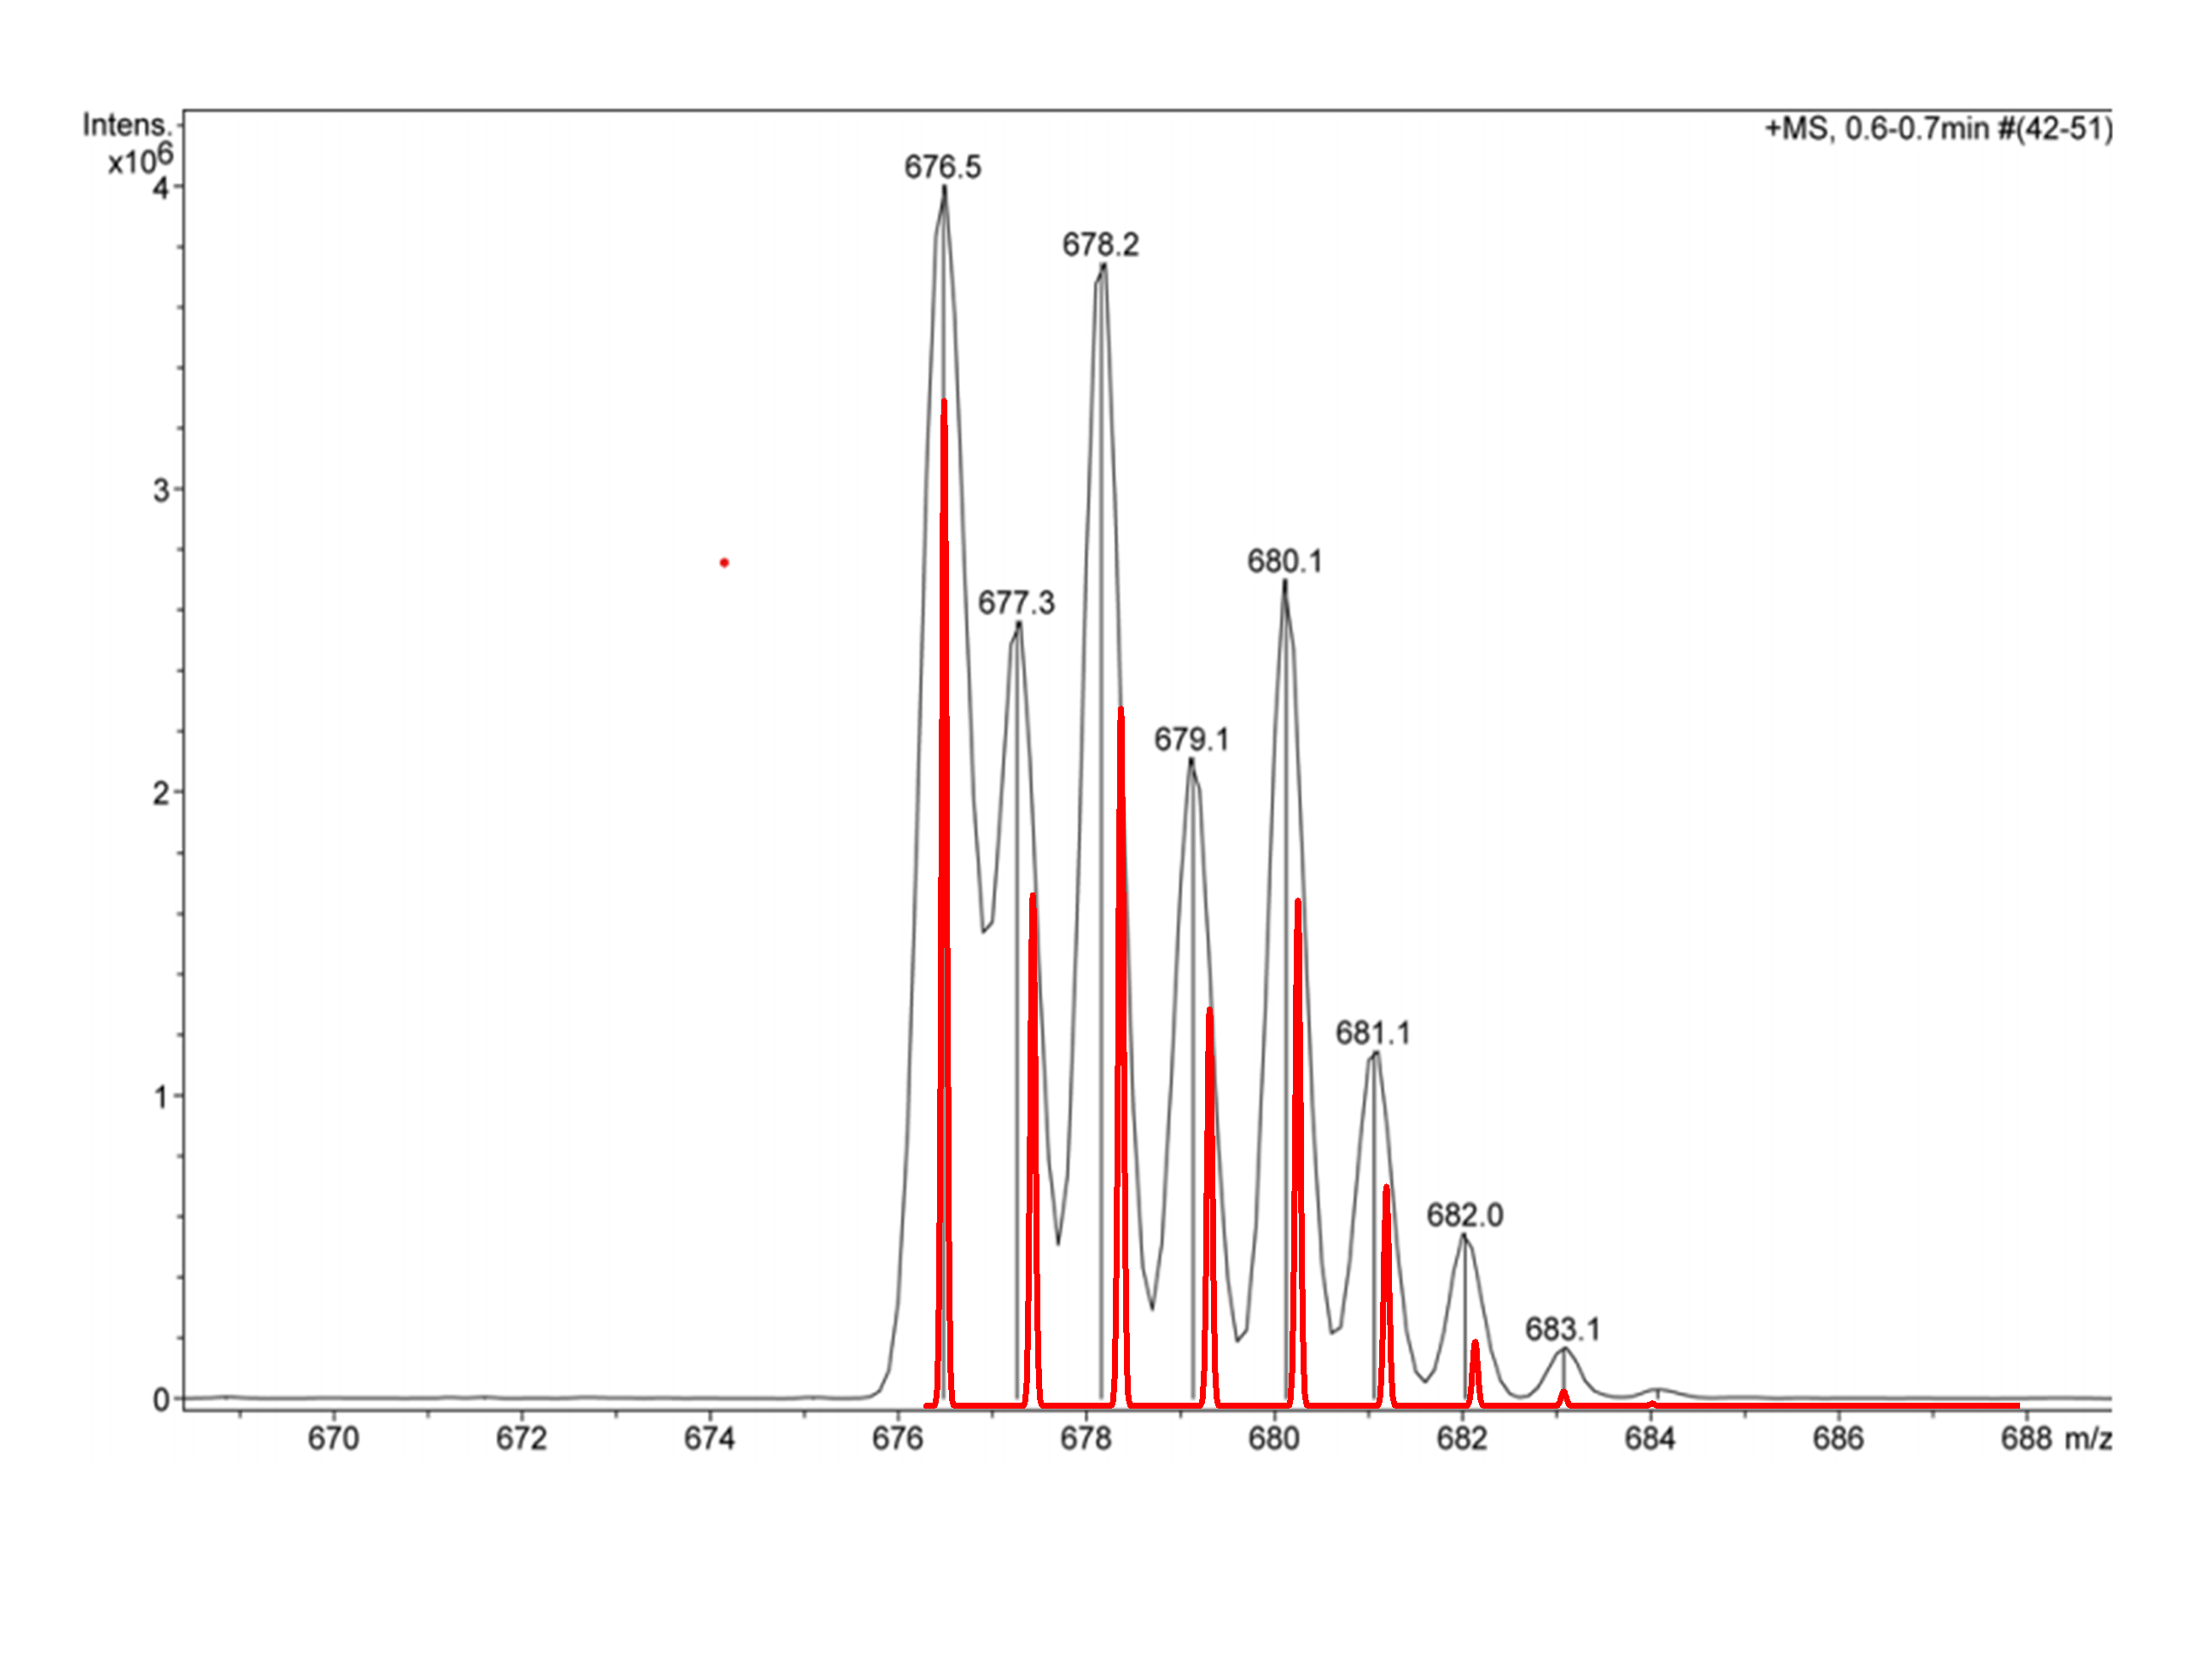
\includegraphics[width=0.5\textwidth]{ESI-MS-Zn-TPP}
        \caption{ESI-MS of Zn-TPP around the main peak corresponding to the unfragmented molecular mass. The predicted spectra is reported as a red line.}
        \label{ESI-MS-Zn-TPP}
    \end{subfigure}
\end{figure}
%%%%%%%%%%%%%%%%%%%%%%%%%%%%%%%%%%%%%%%%%%%%%%%%%%%%%%%%%%%%%%%%%%%%%%
\subsection{Study case}
%Presenting an insightful paper
The wide choice of substitutional groups and the flexibility in metal center coordination that characterize the porphyrinic macrocycle allows the fine tuning of chemistry and optical properties of derived molecules.
In addition, the robustness of the aromatic macrocycle makes the porphyrins the ideal candidate for photochemical applications.\\
A particularly relevant study case discussed by \citet{al_mousawi_zinc_2017} in 2017 reports the effective employment of Zn-TPP as photoinitiator for cationic polymerization.
In the study, the Zn-TPP capabilities as photoinitiator are exploited to engineer photosensitive resins for LED projector 3D printing applications.
In regard to LED projector 3D applications, it is important that the photoinitiator has good stability under air to provide usage flexibility.
Additionally, a desirable photoinitiator has rapid response to exposure to radiation of a specific wavelength, in order to avoid unwanted polymerization.
The optimal photoinitiation wavelength lies in the blue-purple region, since they provide the most energy for effectively promoting an electronic excitation.
However, the most practical reason lies on the fact that the printing run must be supervised.
To do so, the container of the printer must have walls transparent to most of the visible light besides the photoinitiation wavelength.\\

Because of the listed reasons, the porphyrin derivative Zn-TPP is chosen for exhibiting a narrow and intense Soret band (or B band) at 450 nm, thanks to the bathochromic shift induced by the coordinated zinc.
This feature allows for the efficient excitation by wavelengths between 400 nm and 470 nm, see Fig.\ref{UV-Vis-Zn-TPP}.
\begin{figure}
    \centering
    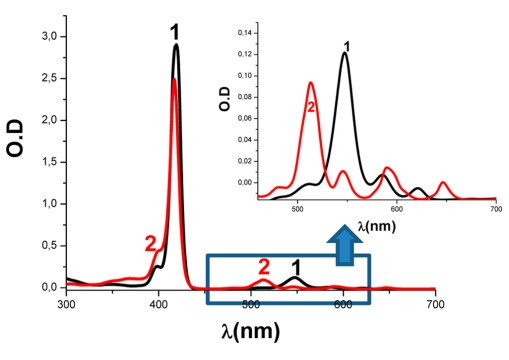
\includegraphics[width=0.3\textwidth]{UV-Vis-Zn-TPP}
    \caption{Absorption spectra in DCM: (1) Zn-TPP; (2) H$_{2}$-TPMP. Reprinted from \citet{al_mousawi_zinc_2017}}
    \label{UV-Vis-Zn-TPP}
\end{figure}
To obtain efficient initiation, the photosensitizer (Zn-TPP) must be combined with an oxidating group like iodonium, in order to effectively strip an electron from the excited Zn-TPP, forming a radical cation, which is able to initiate the polymerization process.
The degree of polymerization is monitored in this study, by the attenuation of characteristic vibrational modes associated to the functional group that undergoes cleavage during the reaction.
The relative residual signal is the complementary of the conversion degree and it is monitored by FTIR in time-wise series to evaluate the kinetic of the polymerization process.
In the reported study, two porhyprins with overlapping optical absorptions (see Fig.\ref{UV-Vis-Zn-TPP}) are compared over their photoinitiating capabilities, highlighting the importance of the metallic center.
Indeed, in Fig. \ref{conv-ZnTPP} it is possible to observe how an higher concentration of photosensitizer fastens the polymerization of the monomer, but the absence of zinc renders the process ineffective.
\begin{figure}
    \centering
    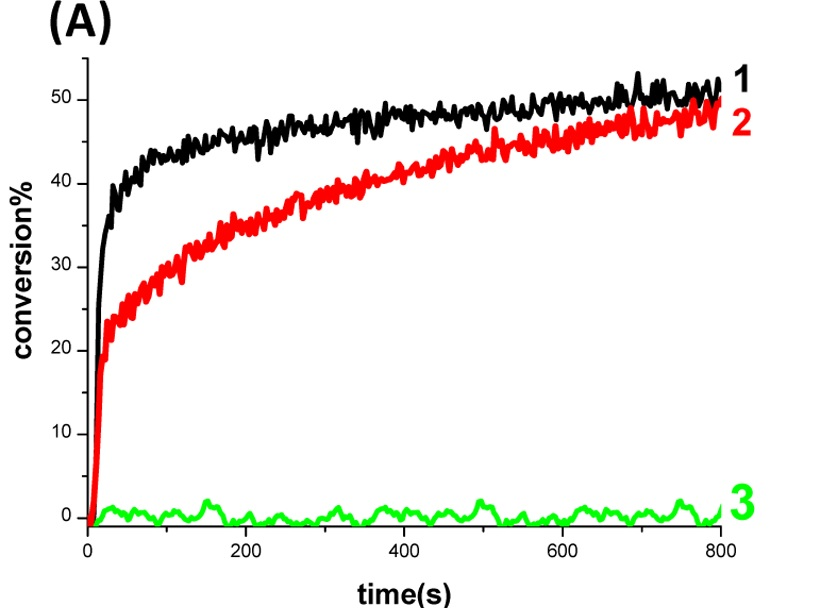
\includegraphics[width=0.3\textwidth]{conv-Zn-TPP}
    \caption{Polymerization profiles (epoxy function conversion vs irradiation time) for EPOX under air (thickness = 25 $\mu$m) upon exposure to
LED@405 nm in the presence of the two-component photoinitiating systems: (1) Zn-TPP/Iod (0.5\%/1\% w/w); (2) Zn-TPP/Iod (0.3\%/1\% w/w);
(3) H$_{2}$-TPMP/Iod (0.5\%/1\% w/w).}
    \label{conv-ZnTPP}
\end{figure}
Finally, it is remarked that the use of photosensitive resins allow for the rapid printing of an entire layer at once due to the absence of a printing head combined with an extremely high resolution, as reporeted in the picture \ref{print}.
\begin{figure}
    \centering
    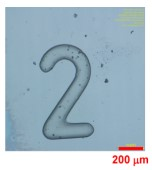
\includegraphics[width=0.3\textwidth]{printed}
    \caption{3D-Photopolymerization experiments using projector LED@ 405 nm.}
    \label{print}
\end{figure}
%%%%%%%%%%%%%%%%%%%%%%%%%%%%%%%%%%%%%%%%%%%%%%%%%%%%%%%%%%%%%%%%%%%%%%%
\section{Conclusions}
It is possible to conclude that despite the simplicity of the synthesis route, the overall yield of the reactions described is remarkably high.
Such promising results are boosted by the intrinsic stabilization of the porphyrin ring and act a fertile ground for the development of alternative synthesis routes that could render the adoption of porhyrins in common applications a likely scenario.
The combination of \textit{in operando} and \textit{ex situ} characterization techniques allowed to speed up the optimization of reaction parameters.
Followingly, a discussion of the general features observed $^{1}$H-NMR and ESI-MS spectra was performed to justify experimental observations performed by credited third parties.
Lastly, an interest use case for Zn-TPP is proposed to reinforce the compelling push towards a clean, fast and cheap synthesis of metallated porhyrins.
%%%%%%%%%%%%%%%%%%%%%%%%%%%%%%%%%%%%%%%%%%%%%%%%%%%%%%%%%%%%%%%%%%%%%%
\section{Experimental}
Reagents were loaded in a round-bottomed flask containing 40 mL of propionic acid.
Firstly, the flask was placed in a heating mantle mounted with an Allihn condenser on top and heated to boil the acid.
The reagents, consisting in 1.65 mL (15.75 mmol) of benzaldehyde and 1 mL of pyrrole (14.4 mmol), were loaded from the upper end of the condenser at the same time to avoid pyrrole polymerization.
Therefore, a small excess of benzaldehyde was used in order to prevent polymerization of the pyrrole into polypyrrole \\
Following, the condenser's walls were wahed with 10 mL of propionic acid to ensure quantitative transfer of the reagents to the flask.
The reaction was driven in reflux conditions for 30 minutes and was monitored through TLC at the beginning and after 30 minutes of reflux.
All the TLCs were performed using as eluent a solution of petroleum ether and ethyl acetate in 3:1 volumetric ratio.
A purple precipitate formed in the flask and upon cooling it was filtered from the solvent.
The filtration was performed using a gootch sieve with a porosity of 3 mounted on Buchner flask connected to a vacuum line.
Subsequently, the solid was washed from propionic acid using methanol, due to the higher volatility of the latter.
The purple crystals, which can be seen in Fig.\ref{pic-tpp}, were removed from the porous sieve with a spatula and transferred into a vial which had been previously weighted.
The product was weighted through the use of a digital scale in order to estimate the reaction yield and a TLC was performed against a commercial standard to ensure successful synthesis.\\
\begin{figure}[h]
    \centering
    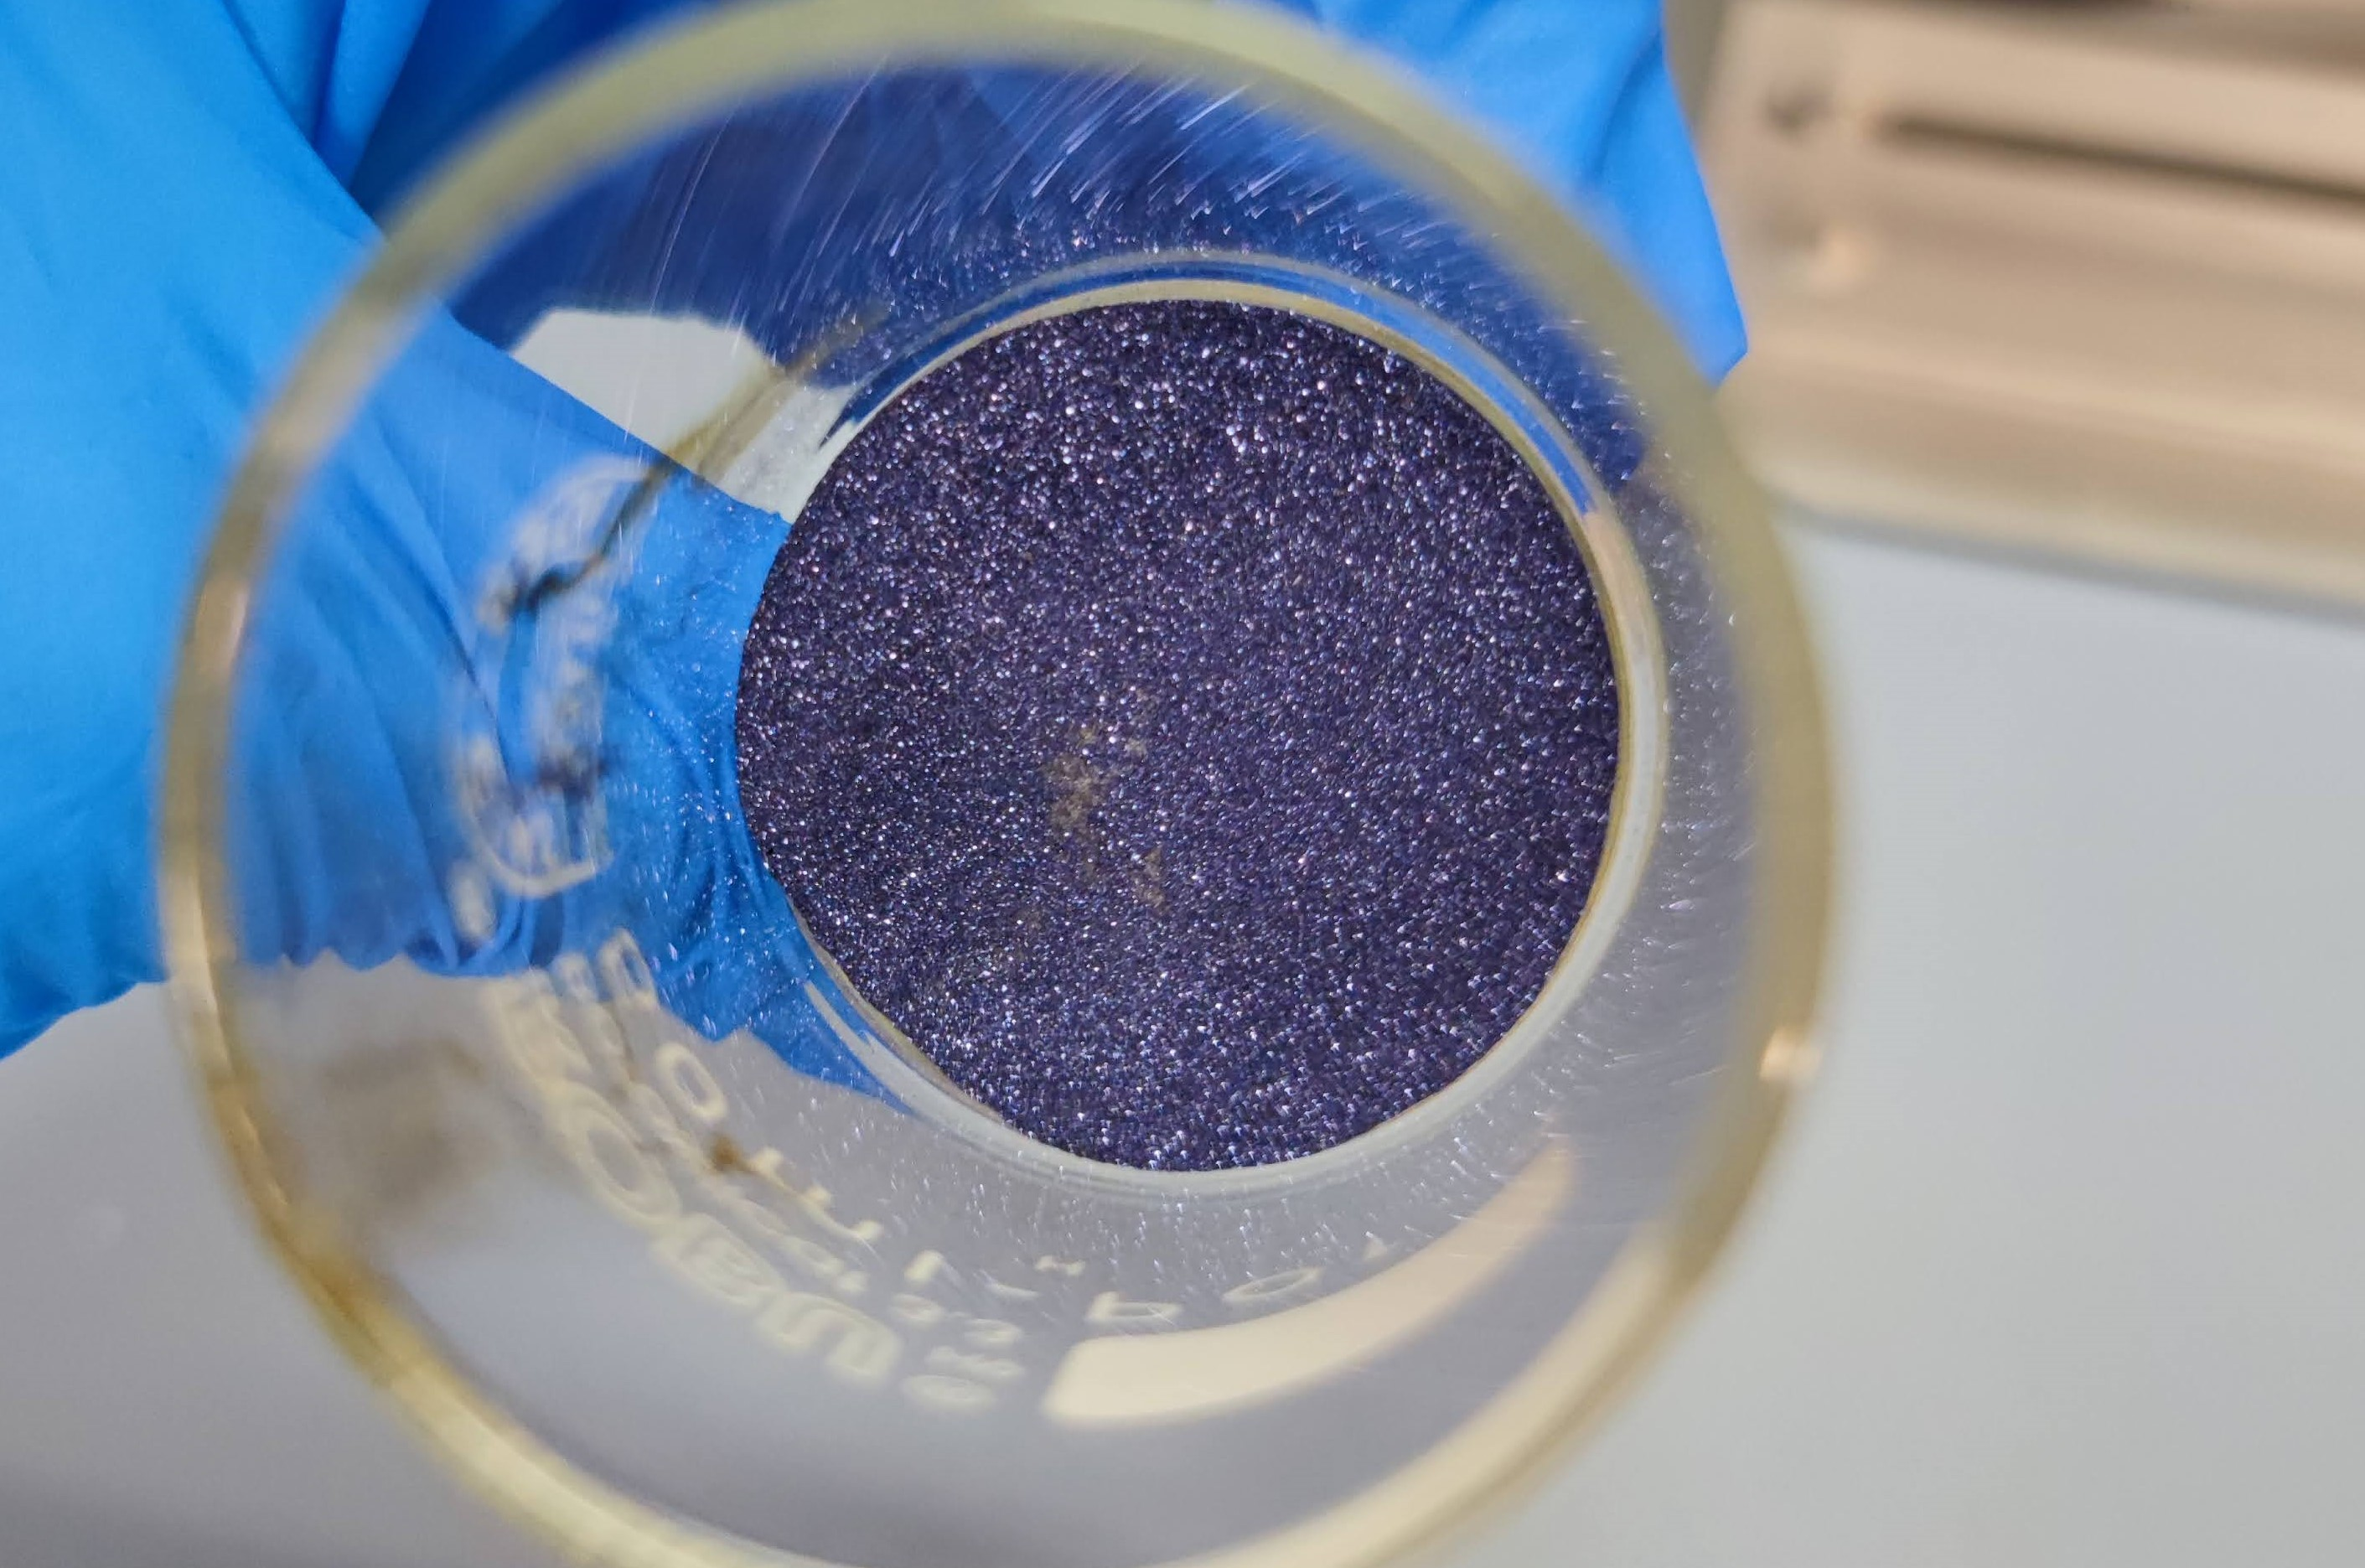
\includegraphics[width=0.4\textwidth]{photo-tpp}
    \caption{Picture portraying the H$_{2}$-TPP crystals collected on the sieve.}
    \label{pic-tpp}
\end{figure}
\break
The metallation of the as-synthesized porphyrin was realized on 160 mg of the sample.
The intermediate product was weighted on a watch glass and then trasferred into a round-bottomed flask alongside with 20 mL of chloroform and heated using a heating mantle.
A volume of 4 mL of a saturated solution of zinc acetate in methanol was then added to the flask and reflux conditions were imposed using an Allihn condenser for 30 minutes.
Also this reaction was monitored through TLC by applying on the plate H$_{2}$-TPP, the starting solution and the reaction solution either after 2, 5 or 25 minutes after mixing the reagents.
In order to avoid the streaking of the spots, the samples from the reaction solution were diluted in chloroform before placing on the TLC plate.\\
\break
At this point, the purification of Zn-TPP is needed in order to separate the product from zinc acetate precursor.
This is achieved through the employment of a separating funnel and use of water as the extracting phase for zinc acetate.
The separation was repeated twice using each time 20 mL of milliQ water.
Furthermore, anhydrification of the chloroform containing Zn-TPP was undertaken by the addition of abundant Na$_{2}$SO$_{4}$ powder.
The sodium sulfate is added until the newly added powder stops aggregating, testifying the lack of water.
The insoluble powder has been filtered from the organic solvent using a paper filter folded to fit in a funnel.
The filtered liquid, containing dissolved Zn-TPP, was collected in a 100 mL round-bottomed flask.
Ultimately, the flask was placed in a rotavapor system to evaporate the solvent and enable the collection of the solid product.
The reaction yield was again estimated by the use of a digital scale and the product was transferred into a vial.\\
The presence of H$_{2}$-TPP and Zn-TPP in the products has been confirmed by ESI-MS, while the purity of the product was qualitatively discussed from $^{1}$H NMR for both the targets.
In both cases, the data was collected by third parties which are mentioned in the respective paragraph.

\section*{acknowledgements}
The contributions of former students in collecting the experimental characterization of their sample has been crucial for validating the synthesis proposed in this work.
\section*{conflict of interest}
The author reports to have a personal interest in the positive outcome of the research work.
\section*{Supporting Information}
A GitHub repository hosts the complete file collection produced as part of this coursework.
It can be found at https://github.com/EC-Finco/Porphyrins-report.
\printendnotes

% Submissions are not required to reflect the precise reference formatting of the journal (use of italics, bold etc.), however it is important that all key elements of each reference are included.
\bibliography{rifporphyrin}
%\graphicalabstract{example-image-1x1}{Please check the journal's author guidelines for whether a graphical abstract, key points, new findings, or other items are required for display in the Table of Contents.}
\end{document}